\DiaryEntry{Game Theory, I}{2023-10-10}{Game Theory}

Based on the book \cite{Maschler2013}.

Game theory uses mathematical tools to model and analyze situations of interactive decision making. The situations involve several decision makers (called players) with different goals, in which the decision of each affects the outcome for all the decision makers.

This interactivity distinguishes game theory from standard decision theory. Game theory tries to predict the behavior of the players and sometimes also provides decision makers with suggestions regarding ways in which they can achieve their goals.

\subsection{Extensive-Form Games}

We need a complete description of a game and this should contain the following elements:

\begin{itemize}
\item A set of players,
\item The possible actions available to each player,
\item Rules determining the order in which players make their moves,
\item A rule determining when the game ends,
\item A rule determining the outcome of every possible game ending.
\end{itemize}

A comprehensive description is by means of a tree where every player’s action is depicted as a transition from one vertex to another vertex.

\paragraph{Example.} As a simple example consider a game with two players, I and II, which play on a 2 x2 gameboard as depicted in the following Figure.

\begin{figure}[H]
    \centering
    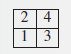
\includegraphics[scale=1.2]{images/2023-10-10-game_theory_01.png}
\end{figure}

Player I has the opening move, in which he "captures" one of the squares. By alternate turns, each player captures one of the squares, subject to the following conditions:

\begin{itemize}
	\item A square may be captured by a player only if it has not been previously captured by either player.
	\item Square 4 may not be captured if square 2 or square 3 has been previously captured.
	\item The game ends when square 1 is captured. The player who captures square 1 is the losing player.
\end{itemize}

Intuitively spoken, each player tries to froce the other to capture square 1 in order to win the game.

We can represent the game in extensive-form with the following graph. Every circled vertex represents a decision by a player, and is labeled with the number of that player. The terminal vertices of the game are indicated by dark dots. The edges of the graph depict game actions. The number that appears next to each edge corresponds to the square that is captured. Next to every terminal vertex, the corresponding game outcome is indicated. A game depicted by such a graph is called a \emph{game in extensive form}, or \emph{extensive-form game}.

\begin{figure}[H]
    \centering
    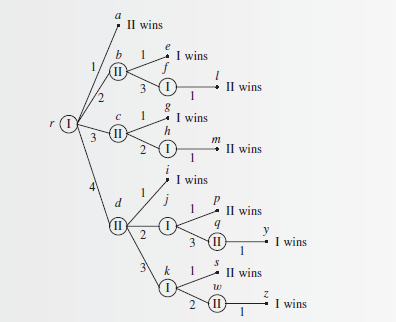
\includegraphics[scale=1.2]{images/2023-10-10-game_theory_02.png}
\end{figure}

The graph starts in vertex $r$ where player I can choose to capture any of the $4$ squares. Chosing square $1$ brings us to vertex $a$ which corresponds to a loss of player I. Chosing square $2$ brings us to vertex $b$ where player II has two options: Either capture square $1$ (vertext $e$) in which case player I wins, or capture square $3$ which brings us to vertex $f$. Here the only option for player I is to capture square $1$ which results in the victory of player II.

Based on above example, we state that various games can be represented by trees: The root of the tree corresponds to the initial position of the game, and every game position is represented by a vertex of the tree. The children of each vertex $v$ are the vertices corresponding to the game positions that can be arrived at from $v$ via one action. In other words, the number of children of a vertex is equal to the number of possible actions in the game position corresponding to that vertex. For every vertex that is not a leaf, we need to specify the player who is to take an action at that vertex. At each leaf, we need to describe the outcome of the game.

\begin{definition}
The formal definition of a game in extensive form is an ordered vector $\Gamma$,

\bee
\Gamma = (N, V, E, x^0, (V_i)_{i \in N}, O, u)
\eee

where

\begin{itemize}
	\item $N$ is finite set of players,
	\item $(V, E, x^0)$ describes the game tree (with vertex set $V$, edge set $E$, and root vertex $x^0$),
	\item $(V_i)_{i \in N}$ is a partition of the set of vertices that are not leaves,
	\item $O$ is the set of possible game outcomes.
	\item $u$ is a function associating every leaf of the tree with a game outcome in the set $O$.
\end{itemize}

\end{definition}

For each player $i \in N$, the set $V_i$ is player $i$’s set of decision vertices. For each leave $x$, the outcome at that leave is $u(x)$.

Note that the partition $V_i$ may contain empty sets. We accept the possibility of empty sets in order to be able to treat games in which a player may not be required to make any moves, but is still a game participant who is affected by the outcome of the game.

In the example game above, the various sets have the following elements

\begin{align*}
N &= \{I, II\}	\\
V &= \{r, a, b, c, d, e, f, g, h, i, j, k, l, m, p, q, s, w, y, z\}	\\
x^0 &= r \\
V_I &= \{r, f, h, j, k\} \\
V_{II} &= \{b, c, d, q, w\}
\end{align*}

The set of possible outcomes is $O = \{I \text{ wins}, II \text{ wins} \}$, and the function $u$ is given by

\begin{align*}
u(a) &= u(l) = u(m) = u(p) = u(s) = \text{ II wins} \\
u(e) &= u(g) = u(i) = u(y) = u(z) = \text{ I wins} \qed
\end{align*}

Finally, denote by $C(x)$ the set of all children of a non-leaf vertex $x$. Every edge that leads from $x$ to one of its children is called a possible action at $x$. We will associate every action with the child to which it is connected, and denote by $A(x)$ the set of all actions that are possible at the vertex $x$.

By definition, the collection of the vertices of the graph is a finite set, so that the game necessarily ends at a leaf, yielding a sequence of vertices $(x^0, x^1, \ldots , x^k)$, where $x^0$ is the root of the tree, $x^k$ is a leaf, and $x^{l+1} \in C(x^l)$ for $l = 0, 1, \ldots k-1$. This sequence is called a play. Every play ends at a particular leaf $x^k$ with outcome $u(x^k)$. Similarly, every leaf $x^k$ determines a unique play, which corresponds to the unique path connecting the root $x^0$ with $x^k$.

It follows from the above description that every player who is to take an action knows the current state of the game, meaning that he knows all the actions in the game that led to the current point in the play. This implicit assumption is called \emph{perfect information}.

Above definitions are for finite games. There are also inifinite games, where the game tree $(V, E, x^0)$ is infinite. This can happen in two possible ways: (i) It is possible that the depth of the tree is bounded, i.e., that there exists a natural number $L$ such that the length of every path in the tree is less than or equal to $L$. This corresponds to a game that ends after at most $L$ actions have been played, and there is at least one player who has an infinite number of actions available at an information set. (ii) It is possible, that the depth of the vertices of the tree is not bounded; that is, there exists an infinite path in the game tree. This corresponds to a game that might never end.


With all these formal definition in place, we can now define one of the central concepts of game theory: the strategy.

\begin{definition}
A strategy for player $i$ is a function $s_i$ mapping each vertex $x \in V_i$ to an element in $A(x)$(equivalently, to an element in $C(x)$).
\end{definition}

According to this definition, a strategy includes instructions on how to behave at each vertex in the game tree, including vertices that previous actions by the player preclude from being reached.

In the example from above, a strategy $s_I$ for player I would define $s_I(x)$ for \emph{all} vertices $x \in V$. Note that this is strictly not necessary for when $s_I(r) = 2$, the play can never reach vertex $j$. So we could omit this and simplify the strategy representation somewhat. So one strategy for player I could be as follows

\bee
s_I(r) = 4, s(j) = 1, s(k) = 2
\eee

When player I choses $4$ in the first move, this brings the play to vertex $d$. Depending on the action player II takes, the play can continue in vertices $i, j,k$. There is no decision necessary when player II has chosen $1$ (player I wins), but in the other two cases, a decision of player I is required.

We next focus on games with two players, I and II, whose set of outcomes is $O = \{I wins, II wins, Draw\}$. We have the following types of strategies.

\begin{definition}
Let $\Gamma$ be an extensive-form game with two players I and II, and with outcome $O = \{I wins, II wins, Draw\}$. A strategy $s_I$ of player I is called a \emph{winning strategy} if

\bee
u(s_I, s_{II}) = I wins, \quad \forall s_{II} \in S_{II}
\eee

A strategy $s_I$ of player I is called a \emph{strategy guaranteeing at least a draw} for player II if

\bee
u(s_I, s_{II}) \in \{I wins, Draw\}, \quad \forall s_{II} \in S_{II}
\eee
\end{definition}

We have the following theorem.

\begin{theorem}
\label{2023-10-10-th1}
In every two-player game (with perfect information) in which the set of outcomes is $O = \{I wins, II wins, Draw\}$, one and only one of the following three alternatives holds:

\begin{itemize}
	\item Player I has a winning strategy.
	\item Player II has a winning strategy.
	\item Each of the two players has a strategy guaranteeing at least a draw.	
\end{itemize}

\end{theorem}


\subsubsection{Games with Chance Moves}

So far, the transition from one state to another has always been controlled by actions undertaken by the players. However, there are games where random events are part o the game (such as rolling a dice). To accommodate this feature, the model is expanded by labeling some of the vertices in the game tree $(V,E, x^0)$ as chance moves. The edges emanating from vertices corresponding to chance moves represent the possible outcomes of a lottery, and next to each such edge is listed the probability that the outcome it represents will be the result of the lottery.

Formally, we handle chance moves by adding another player denoted by $0$ (so in total, the players become $N \cup 0$). For every vertex $x$ at which a chance move is implemented, we denote by $p_x$ the probability vector over the possible outcomes of a lottery that is implemented at vertex $x$.

\begin{definition}
The formal definition of a game with chance moves is now given by

\bee
\Gamma = (N, V, E, x^0, (V_i)_{i \in N \cup 0}, (p_x)_{x \in V_0}, O, u)
\eee
	
\end{definition}

The following Figure shows a game with chance moves. The outcomes of the game are noted by pairs of numbers $(z_I, z_{II})$, where $z_I$ is themonetary payoff to Player I, and $z_{II}$ is the monetary payoff to Player II.

Player I starts with the choice of selecting between action a, which leads to the termination of the game with payoff
$(0, 0)$, and action b, which leads to a chance move at vertex A. The chance move is a lottery (or a flip of a coin) leading with probability $1/2$ to state B, which is a decision vertex of Player II, and with probability $1/2$ to state C, which is a decision vertex of Player I.

At state B, Player II chooses between action f , leading to a termination of the game with payoff $(2,0)$, and action e leading to
state D which is a chance move; at this chance move, with probability $1/3$ the game ends with payoff $(5,-1)$, and with probability $2/3$ the game ends with payoff $(-2,5)$. At state C, Player I chooses between action g, leading to the termination of the game with payoff $(1,1)$, and action h, leading to a chance move at vertex E. At this chance move the game ends, with payoff $(0,2)$, or $(-1,1)$, or $(1,1)$, with respective probabilities $1/4$, $1/2$, and $1/4$.


\begin{figure}[H]
    \centering
    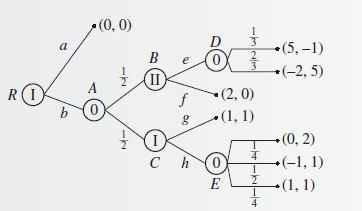
\includegraphics[scale=1.2]{images/2023-10-10-game_theory_03.png}
\end{figure}


Note that there is a hidden assumption, that the probabilities of the chance moves are known to all the players. More advanced models take into account the possibility that the players do not all necessarily share the same assessments of the probabilities of chance moves, but these will be discussed later.

Continuing with our example, let's assume that player I uses strategy $s_I$ defined as

\bee
s_I(R) = b, s_I(C) = h
\eee

and player II follows the strategy $s_{II}$ defined as

\bee
s_{II}(B) = f
\eee

Following these strategies, the following paths are possible

\begin{align*}
1:& R \rightarrow A \rightarrow B \rightarrow (2,0) \\
2:& R \rightarrow A \rightarrow C \rightarrow E \rightarrow (0,2) \\
3:& R \rightarrow A \rightarrow C \rightarrow E \rightarrow (-1,1) \\
4:& R \rightarrow A \rightarrow C \rightarrow E \rightarrow (1,1)
\end{align*}

The probablities $p_i$ for these plays are given by multiplying the probabilities of each chance moves as

\bee
p_1 = \frac{1}{2}, \quad p_2 = \frac{1}{2} \cdot \frac{1}{4} = \frac{1}{8}, \quad p_3 = \frac{1}{2} \cdot  \frac{1}{2} = \frac{1}{4}, \quad p_4 = \frac{1}{2} \cdot \frac{1}{4} = \frac{1}{8}
\eee

Note that von Neumann’s Theorem (\ref{2023-10-10-th1}) does not hold in games with chance moves. In dice games, such as backgammon, a player who benefits from favorable rolls of the dice can win regardless of whether or not he has the first move, and regardless of the strategy adopted by his opponent.

\subsubsection{Games with Imperfect Information}

So far in every stage of the game each of the players has perfect knowledge of all the developments in the game prior to that stage: he knows exactly which actions were taken by all the other players, and if there were chance moves, he knows what the results of the chance moves were. In other words, every player, when it is his turn to take an action, knows precisely at which
vertex in the game tree the game is currently at. A game satisfying this condition is called a \emph{game with perfect information}.

We can remedy this and consider \emph{games with imperfect information} by introducing \emph{information sets}: A player’s information set consists of a set of vertices that when play reaches one of these vertices, the player knows that play has reached one of these vertices, but he does not know which vertex has been reached.

As an example, consider the following game with two players in which each player chooses one of the sides of a coin, H (for heads) or T (for tails) in the following way: each player inserts into an envelope a slip of paper on which his choice is written. The envelopes are sealed and submitted to a referee. If both players have selected the same side of the coin, Player II pays one dollar to Player I. If they have selected opposite sides of the coin, Player I pays one dollar to Player II.

The information set is depicted by means of an ellipse: The two vertices A and B of Player II are surrounded by an ellipse which indicates that when Player II is in the position of selecting between h and t, he does not know whether the game state is currently at vertex A or vertex B, because he does not know whether Player I has selected H or T . These two vertices together form an information set of Player II.

\begin{figure}[H]
    \centering
    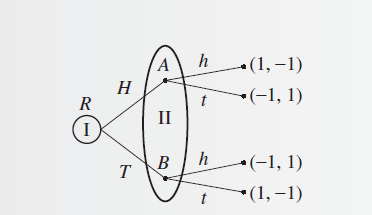
\includegraphics[scale=1]{images/2023-10-10-game_theory_04.png}
\end{figure}

Note: Above graph suggests that player I starts with his choice and then player II decides (being not aware of player I's decision). According to the game description, both players decide at the same time. However, using imperfect information, we can model the concurent decision by means of a sequential model. We could also have reversed the order of player I and II and achieved the same result.

With imperfect information, a strategy looks slightly different. For player I, the strategy needs to define what to do at vertex $R$ (eg $s_I(R) = H$). However, for player II we can only state what to do in the information set (let's call it $AB$); $s_{II}(AB) = h$.


\subsection{Strategic-Form Games}

The strategic-form description ignores dynamic aspects of the game, such as the order of the moves by the players, chance moves, and the informational structure of the game. Instead, a game in strategic form consists of a set of players, a strategy set for each player, and an outcome to each vector of strategies, which is usually given by the vector of utilities the players enjoy from the outcome. This allows to focus on which strategies are more likely to be played by the players, or to recommend to players which strategy to implement (or not to implement).

\paragraph{Example Rock-Paper-Scissor.} The two players select simultaneously one of the three options. The outcome is determined by the following rules: rock smashes scissors, scissors cut paper, paper covers rock. This is shown in the following Figure. Note the big ellipse representing the information set of player II as he does not know what player I has selected.

\begin{figure}[H]
    \centering
    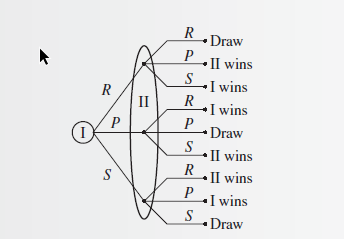
\includegraphics[scale=1]{images/2023-10-10-game_theory_05.png}
\end{figure}

Setting the payoff to a player to be $1$ for a win, $-1$ or a loss, and $0$ for a draw, we obtain the game in strategic form as shown in the Figure below. In each cell the left number denotes the payoff to Player I and the right number denotes the payoff to Player II.

Note: Fig. 4.4 in the book \cite{Maschler2013} is wrong; below is the corrected one.

\begin{figure}[H]
    \centering
    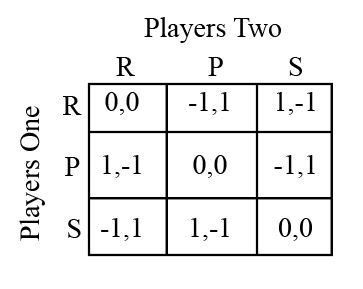
\includegraphics[scale=0.7]{images/2023-10-10-game_theory_06.png}
\end{figure}



\paragraph{Example 2.} This example is a game with perfect information. Player I has two strategies: He can choose between U(p) and D(own) in the first move,

\bee
s_{I,1}(R) = U, \quad s_{I,2}(R) = D
\eee

Having observed player I's decision, player II can decide between R(ight) and L(eft), leaving him with four strategies:

\begin{itemize}
	\item $s_{II,1}$: Chose R when player I has chosen U, chose R when player I has chosen D (aka always chose R), $s_{II,1}(U) = R, s_{II,1}(D) = R$. We will abbreviate this with "R,R".
	\item $s_{II,2}$: Chose R when player I has chosen U, chose L when player I has chosen D, $s_{II,2}(U) = R, s_{II,2}(D) = L$. We will abbreviate this with "R,L".
	\item $s_{II,3}$: Chose L when player I has chosen U, chose R when player I has chosen D, $s_{II,3}(U) = L, s_{II,3}(D) = R$. We will abbreviate this with "L,R".
	\item $s_{II,4}$: Chose L when player I has chosen U, chose L when player I has chosen D (aka always chose L), $s_{II,4}(U) = L, s_{II,4}(D) = L$. We will abbreviate this with "L,L".
\end{itemize}

The following Figure shows the extensive-form game and the table below the strategic-form game. One has to be a bit careful with correctly interpreting the table and differentiating between a strategy and a decision.

The upper left field at "coordinates" U-R,L with payoff $5,2$ corresponds to the case that player I chose U and player II strategy $s_2$ yields an action of R, $s_2(U) = R$. According to the extensive-form representation, this corresponds to a payoff of $5,2$; the corresponding play is shown in red in the Figure. 

Note that the field at "coordinates" U-R,R yields the same $5,2$ payoff: Although the strategy is different, namely $s_1$, it yields the same action, $s_1(U) = R$, and therefore the payoff is the same.

\begin{figure}[H]
    \centering
    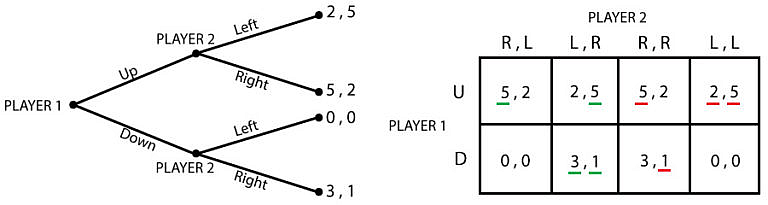
\includegraphics[scale=0.5]{images/2023-10-10-game_theory_07.png}
\end{figure}

\begin{table}[H]
	\begin{tabular}{llllll}
		&   & \multicolumn{4}{c}{Player 2}                                      \\ \cline{2-6} 
\multicolumn{1}{l|}{}                           &   & R,L                        & L,R & R,R & \multicolumn{1}{l|}{L,L} \\ \cline{2-6} 
\multicolumn{1}{c|}{}                           & U & {\color[HTML]{FE0000} 5,2} & 2,5 & 5,2 & \multicolumn{1}{l|}{2,5} \\
\multicolumn{1}{c|}{\multirow{-2}{*}{Player 1}} & D & 0,0                        & 3,1 & 3,1 & \multicolumn{1}{l|}{0,0} \\ \cline{2-6} 
\end{tabular}
\end{table}

When there are no chance moves, a game in strategic form is derived from a game in extensive form in the following way:

\begin{itemize}
	\item List the set of all strategies $S_i$ available to each player $i$ in the extensive-form game.
	\item For each vector $s$ of strategies find the play determined by this vector of strategies, and then derive the payoffs induced by this play, $u_1(s), u_2(s), \ldots, u_n(s)$.
	\item Draw the appropriate n-dimensional matrix. When there are two players, the number of rows in the matrix equals the number of strategies of Player I, the number of columns equals the number of strategies of Player II, and the pair of numbers appearing in each cell is the pair of payoffs defined by the pair of strategies associated with that cell. When there are more than two players, the matrix is multi-dimensional.
\end{itemize}

\subsection{Domination}

We first introduce some new notation: Suppose we have an length-$n$ vector $x = (x_1, \ldots, x_n)$ and by omitting the $i$-th element, we obtain a length-$n-1$ vector which we denotes as $x_{-i} = (x_1, \ldots, x_{i-1}, x_{i+1}, \ldots x_n)$. We define the cartesian product of $n$ sets, $X_1 \times X_2 \ldots X_n = \prod_{i \in N} X_i$ where $N = \{1,2, \ldots, n\}$. Analogously, we define the cartesian product of all but the $i$-th set as $X_{- i} = \prod_{j \neq i} X_j$.

We have now two ways to describe a game: By means of extensive form and by means of the strategic-form. We now tackle the question what can we expect to happen when such a game is played? What outcomes, or set of outcomes, will reasonably ensue, given certain assumptions regarding the behavior of the players?

\paragraph{Example.} Consider the following strategic-form game shown in the following Figure.

\begin{figure}[H]
    \centering
    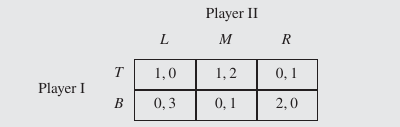
\includegraphics[scale=0.75]{images/2023-10-10-game_theory_10.png}
\end{figure}

Player I has two strategies, T and B, whereas player II has three strategies, L, M, and R. Let's compare player II's stategies M and R:

\begin{itemize}
	\item If Player I plays T , the payoff to Player II under strategy M is $2$, compared to only $1$ under strategy R.
	\item If Player I plays B, the payoff to Player II under strategy M is $1$, compared to only $0$ under strategy R.
\end{itemize}

We see that independently of whichever strategy is played by Player I, strategy M always yields a higher payoff to Player II than strategy R. This motivates the following definition.

\begin{definition}
A strategy $s_i$ of player $i$ is strictly dominated if there exists another strategy $t_i$ of player $i$ such that for each strategy vector $s_{-i} \in S_{-i}$ of the other players,

\bee
u_i(s_i , s_{-i}) < u_i (t_i , s_{-i} )
\eee

If this is the case, we say that $s_i$ is strictly dominated by $t_i$ , or that $t_i$ strictly dominates $s_i$.
\end{definition}

In the previous example strategy R is strictly dominated by strategy M. It is therefore reasonable to assume that if Player II is “rational,” he will not choose R, because under any scenario in which he might consider selecting R, the strategy M would be a better choice.

In the following, there is a lengthy discussion about player rationality and that all players know that the others are rational and all players know that all players know that all players are rational. The summary is that the fact that all players are rational is common knowledge among the players and strictly dominated strategies can be eliminated under this assumption.

Elimination of strategy $R$ leads to the following strategic-form game.

\begin{figure}[H]
    \centering
    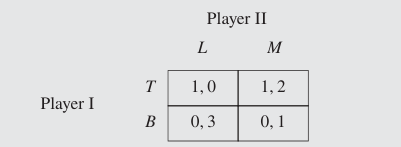
\includegraphics[scale=0.75]{images/2023-10-10-game_theory_11.png}
\end{figure}

However, we can continue to search for dominated stategies: We find that for player I it is always better to play strategy T than strategy B, so we can eliminate this one as well. We finally arrive at the following strategic-form game.

\begin{figure}[H]
    \centering
    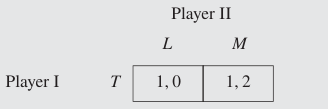
\includegraphics[scale=0.75]{images/2023-10-10-game_theory_12.png}
\end{figure}

And - finally - we see that strategy M is better for player II than strategy L. After elimination of L only one result remains, namely $(1, 2)$, which is obtained when Player I plays T and Player II plays M.

The process we have just described is called \emph{iterated elimination of strictly dominated strategies}. When this process yields a single strategy vector (one strategy per player), as in the example above, then, under the assumption of common knowledge of rationalityof all players, the resulting strategy vector can be regarded as the solution of the game.

A special case in which such a solution is guaranteed to exist is the family of games in which every player has a strategy that strictly dominates all of his other strategies, that is, a \emph{strictly dominant strategy}. Clearly, in that case, the elimination of all strictly dominated strategies leaves each player with only one strategy: his strictly dominant strategy. When this occurs we say that the game has a solution in \emph{strictly dominant strategies}.

\paragraph{Prisoner's Dilemma.}\label{2023-10-10_pd} Two individuals who have committed a serious crime are apprehended. Lacking incriminating evidence, the prosecution can obtain an indictment only by persuading one (or both) of the prisoners to confess to the crime. Interrogators give each of the prisoners – both of whom are isolated in separate cells and unable to communicate with each other – the following choices:

\begin{itemize}
	\item If you confess and your friend refuses to confess, you will be released from custody and receive immunity as a state’s witness.
	\item If you refuse to confess and your friend confesses, you will receive the maximum penalty for your crime (ten years of prison).
	\item If both of you sit tight and refuse to confess, we will make use of evidence that you have committed tax evasion to ensure that both of you are sentenced to a year in prison.
	\item If both of you confess, it will count in your favor and we will reduce each of your prison terms to six years.
\end{itemize}

This situation defines a two-player strategic-form game in which each player has two strategies: D, which stands for Defection, betraying your fellow criminal by confessing, and C, which stands for Cooperation, cooperating with your fellow criminal and not confessing the crime. Using this notation,the outcome of the game is summarized in the table below.

\begin{figure}[H]
    \centering
    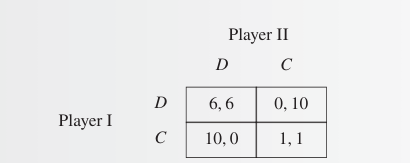
\includegraphics[scale=0.75]{images/2023-10-10-game_theory_20.png}
\end{figure}

Assume player I cooperates (choses strategy C). If player II does the same, player I and player II will go one year into prison (lower right corner). However, player II can improve his situation by chosing to defect, thereby avoiding jail at all. In this case, player I will go to jail for 10 years. Since player I knows this, he will not chose strategy C but D; in the worst case, he will go to jail for 6 years (when player II choses D). That's actually the optimum for player II, so both of them will chose strategy D, causing them to go to prison for 6 years.

So while strategy $(C,C)$ yields the optimum for both player, it is not \emph{stable}: If one player deviates, he can improve his situation (and worsening the situation for the other). Therefore the players will not chose strategy C but D which leads to a worse outcome, but a stable one. \qed


In the Prisoner's dilemma, two strictly dominated strategies were eliminated (one per player), but there was no specification regarding the order in which these strategies were eliminated: was Player I’s strategy C eliminated first, or Player II’s, or were they both eliminated simultaneously? It turns out that the order of elimination makes no difference. It turns out that this is a general result: whenever iterated elimination of strictly dominated strategies leads to a single strategy vector, that outcome is independent of the order of elimination. In fact, we can make an even stronger statement: even if iterated elimination of strictly dominated strategies yields a set of strategies (not necessarily a single strategy), that set does not depend on the order of elimination.

There are games in which iterated elimination of strictly dominated strategies does not yield a single strategy vector. For example, in a game that has no strictly dominated strategies, the process fails to eliminate any strategy.

Such a game is shown in the following Figure: There are no strictly dominated strategies in this game, however, strategy B has a special attribute: although it does not always guarantee a higher payoff to Player I relative to strategy T , in all cases it does grant him a payoff at least as high, and in the special case in which Player II chooses strategy L, B is a strictly better choice than T . In this case we say that strategy B weakly dominates strategy T (and strategy T is weakly dominated by strategy B).

\begin{figure}[H]
    \centering
    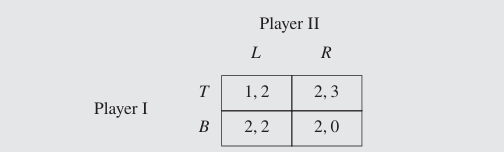
\includegraphics[scale=0.75]{images/2023-10-10-game_theory_21.png}
\end{figure}

\begin{definition}
Strategy $s_i$ of player $i$ is termed weakly dominated if there exists another strategy $t_i$ of player $i$ satisfying the following two conditions: 

\begin{itemize}
	\item For every strategy vector $s_{-i} \in S_{-i}$ of the other players,
	\bee
	u_i(s_i, s_{-i}) \leq u_i(t_i, s_{-i})
	\eee

	\item There exists a strategy vector $t_{-i} \in S_{-i}$ of the other players such that
	\bee
	u_i(s_i, t_{-i}) < u_i(t_i, t_{-i})
	\eee
\end{itemize}

In this case we say that strategy $s_i$ is weakly dominated by strategy $t_i$, and that strategy $t_i$ weakly dominates strategy $s_i$.
\end{definition}

If strategy $t_i$ dominates (weakly or strictly) strategy $s_i$, then $s_i$ does not (weakly or strictly) dominate $t_i$. Clearly, strict domination implies weak domination. Because we will refer henceforth almost exclusively to weak domination, we use the term “domination” to mean “weak domination,” unless the term “strict domination” is explicitly used.

We furthermore assume that a rational player does not use a dominated strategy.

Under this assumption we can eliminate strategy T (as it is weakly dominated), and then proceed to eliminate strategy R (which
is strictly dominated after the elimination of T ). The only remaining strategy vector is (B, L), with a payoff of $(2, 2)$. Such a strategy vector is called \emph{rational}, and the process of iterative elimination of weakly dominated strategies is called \emph{rationalizability}. The meaning of “rationalizability” is that a player who expects a certain strategy vector to obtain can explain to himself why that strategy vector will be reached, based on the assumption of rationality.

\begin{definition}
A strategy vector $s \in S$ is termed rational if it is the unique result of a process of iterative elimination of weakly dominated strategies.
\end{definition}

Note: While the elimation order of strictly dominated strategies does not matter, the elimination order of weakly dominated strategies may matter. In the book, this is demonstrated in example 4.16.

\subsection{Stability: Nash Equilibrium}

As motivating example, we consider the following two-player game in strategic form.

\begin{figure}[H]
    \centering
    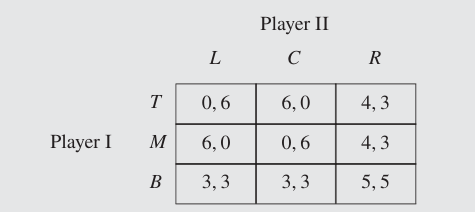
\includegraphics[scale=0.75]{images/2023-10-10-game_theory_30.png}
\end{figure}


There is no dominance relationship between the strategies in this game: For example, if we compare the strategies T and M of Player I, it turns out that neither of them is always preferable to the other: M is better than T if Player II chooses L, and T is better than M if Player II chooses C. In fact, M is the best reply of Player I to L, while T is his best reply to C, and B is his best reply to R. Similarly, for Player II, L is the best reply to T and C
is the best reply to M, while strategy R is the best reply to B.

However, if a player knows which strategy the other player(s) are going to choose, he will choose the best reply to those strategies used by the other players. In our example, this is as follows,

\begin{itemize}
	\item If Player II knows that Player I will choose T , he will choose L (his best reply to T ).
	\item If Player I knows that Player II will choose L, he will choose M (his best reply to L).
	\item If Player II knows that Player I will choose M, he will choose C (his best reply to M).
	\item If Player I knows that Player II will choose C, he will choose T (his best reply to C).
	\item If Player II knows that Player I will choose B, he will choose R (his best reply to B).
\end{itemize}

The pair of strategies (B, R) satisfies a stability property: each strategy in this pair is the best reply to the other strategy. Alternatively, we can state this property in the following way: assuming the players choose (B, R), neither player has a profitable deviation; that is, under the assumption that the other player indeed chooses his strategy according to (B, R), neither player has a strategy that grants a higher payoff than sticking to (B, R).

This stability property is called a \emph{Nash equilibrium} and formally defined as follows.

\begin{definition}
	A strategy vector $s^\star = (s^star_1, \ldots, s^\star_n)$ is a Nash equilibrium if for each player $i \in N$ and each strategy $s_i \in S_i$ the following is satisfied:
	
	\bee
		u_i(s^\star) \geq u_i(s_i, s^\star_{- i})
	\eee

	The payoff vector $u(s^\star)$ is the equilibrium payoff corresponding to the Nash equilibrium $s^\star$.
\end{definition}

We can define a Nash equilibrium also in terms of a \emph{profitable deviation}. The strategy $\hat{s}_i \in S_i$ is a profitable deviation of player $i$ at a strategy vector $s \in S$ if $u_i(\hat{s}_i, s_{-i}) > u_i(s)$. A Nash equilibrium is a strategy vector at which no player has a profitable deviation.

The Nash equilibrium $s^\star$ is often simply referred to as an equilibrium, and sometimes as an equilibrium point. As defined above, it says that no player $i$ has a profitable unilateral deviation from $s^\star$.

The Nash equilibrium can also be equivalently expressed in terms of the best-reply concept.

\begin{definition}
Let $s_{-i}$ be a strategy vector of all the players not including player $i$. Player $i$’s strategy $s_i$ is termed a best reply to $s_{-i}$ if

\bee
u_i(s_i, s_{-i}) = \max_{t_i \in S_i} u_i(t_i, s_{-i})
\eee

\end{definition}

Then we can define the Nash equilibrium in an equivalent manner as follows.

\begin{definition}
The strategy vector $s^\star = (s^\star_1, \ldots, s^\star_n)$ is a Nash equilibrium if $s^\star_i$ is a best reply to $s^\star_{-i}$ for every player $i \in N$.
\end{definition}

As a last practical definition, we can define a Nash equilibrium for two person games as follows: If the first payoff number, in the payoff pair of the cell, is the maximum of the column of the cell and if the second number is the maximum of the row of the cell - then the cell represents a Nash equilibrium.


In the running example, we can use this last definition to verify that (B,R) is the unique Nash equilibrium. For example, the pair (T, L) is not an equilibrium, because T is not a best reply to L; Player I has a profitable deviation from T to M or to B. Out of all the nine strategy pairs, (B, R) is the only equilibrium.

In case of the prisoner's dilemma, \ref{2023-10-10_pd}, there is one equilibrium (D, D), in which both prisoners confess to the crime, resulting in
payoff (1, 1). 


As another example, consider a \emph{coordination game}: Two players can choose two stragegies, and they get a payoff, if they chose the same strategy. The following Figure shows an example for such a game.

\begin{figure}[H]
    \centering
    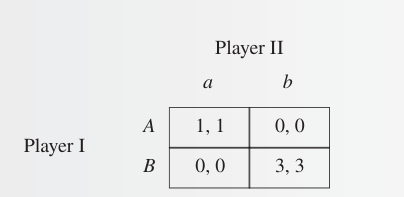
\includegraphics[scale=0.75]{images/2023-10-10-game_theory_31.png}
\end{figure}

Here, both (A, a) and (B, b) are equilibrium points. The equilibrium payoff associated with (A, a) is (1, 1), and the equilibrium payoff of (B, b) is (3, 3). In both cases, and for both players, the payoff is better than (0, 0), which is the payoff for “miscoordinated” strategies (A, b) or (B, a).


\subsection{The Max-min Concept}

As motivating example, consider the following two-person game.

\begin{figure}[H]
    \centering
    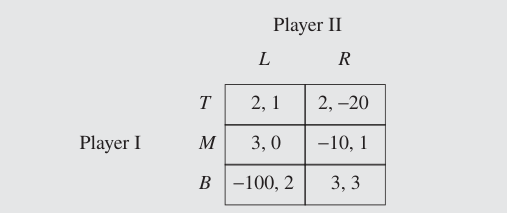
\includegraphics[scale=0.75]{images/2023-10-10-game_theory_40.png}
\end{figure}

According to the above, it has a unique equilibrium for the strategy pair (B,R), with a payoff of (3,3). However, it is not sure whether this equilibrium will really be chosen. Player I would hesitate choosing B: What if Player II were to choose L (whether by accident, due to irrationality, or for any other reason)? The result (B, L) is catastrophic for Player I, so he may prefer strategy T, which guarantees a payoff of only 2 (compared to the equilibrium payoff of 3), but also guarantees that he will avoid getting -100 instead. If Player II is aware of this hesitation, and believes that there is a reasonable chance that Player I will flee to the safety of T, he will also be wary of choosing the equilibrium strategy R (and risking the -20 payoff), and will likely choose strategy L instead. This, in turn, increases Player I’s motivation to choose T.

From player i's point if view, if he chooses strategy $s_i$, the worst possible payoff he can get is

\bee
\min_{t_{-i} \in S_{-i}} u_i(s_i, t_{-i})
\eee

Player $i$ can then choose the strategy $s_i$ that maximizes this value. In other words, disregarding the possible rationality (or irrationality) of the other players, he can guarantee for himself a payoff of

\bee
\underline{v}_i = \max_{s_i \in S_i} \min_{t_{-i} \in S_{-i}} u_i(s_i, t_{-i})
\eee

The quantity $\underline{v}_i$ is called the \emph{maxmin value} of player $i$ or player $i$'s security level. A strategy $s^\star_i$ that guarantees this value is called a \emph{maxmin strategy} and satisfies

\bee
\min_{t_{-i} \in S_{-i}} u_i(s^\star_i, t_{-i}) \geq \min_{t_{-i} \in S_{-i}} u_i(s_i, t_{-i}), \quad \forall s_i \in S_i
\eee

which is equvalent to

\bee
\min_{t_{-i} \in S_{-i}} u_i(s^\star_i, t_{-i}) \geq \underline{v}_i , \quad \forall t_{-i} \in S_{-i}
\eee

For the runing example, the following Figure additionally shows the the worst payoff to Player I if he chooses the strategy of the corresponding row in the right-most column (outside the payoff matrix). Similarly, the numbers in the bottom-most row (outside the payoff matrix) indicate the worst payoff to Player II if he chooses the strategy of the corresponding column. Finally, the oval contains the maxmin value of both players.

\begin{figure}[H]
    \centering
    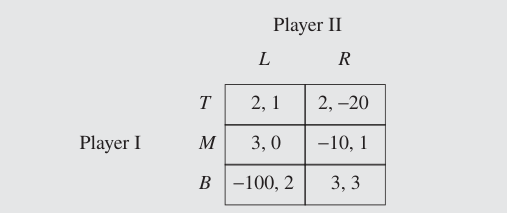
\includegraphics[scale=0.75]{images/2023-10-10-game_theory_40.png}
\end{figure}

The maxmin value of Player I is 2 and the strategy that guarantees this value is T. The maxmin value of Player II is 0 with maxmin strategy L. If the two players choose their maxmin strategies, the result is (T, L) with payoff (2, 1), in which Player II’s payoff of 1 is greater than his maxmin value.

There are some connections between the maxmin strategy and dominant strategies.

\begin{theorem}
A strategy of player $i$ that dominates all his other strategies is a maxmin strategy for that player. Such a strategy, furthermore, is a best reply of player $i$ to any strategy vector of the other players.	
\end{theorem}

From this we obtain the following conclusions.

\begin{theorem}
In a game in which every player has a strategy that dominates all of his other strategies, the vector of dominant strategies is an equilibrium point and a vector of maxmin strategies.

In a game in which every player $i$ has a strategy $s^\star_i$ that strictly dominates all of his other strategies, the strategy vector $(s^\star_1, \ldots, s^\star_n)$ is the unique equilibrium point of the game as well as the unique vector of maxmin strategies.
\end{theorem}

The next theorem establishes a connection between the maxmin value of a player and his payoff in a Nash equilibrium.

\begin{theorem}
Every Nash equilibrium $\sigma^\star$ of a strategic-form game satisfies $u_i(\sigma^\star) \geq \underline{v}_i$ for every player $i$.	
\end{theorem}

\subsection{Two-player zero-sum games}

The Nash equilibrium and the maxmin are two different concepts that reflect different behavioral aspects: the first is an expression of stability, while the second captures the notion of security. Despite the different roots of the two concepts, there are cases in which both lead to the same results. A special case where this occurs is in the class of two-player zero-sum games.

In a given two-player game, denote, as we have done so far, the set of players by $N = \{I, II\}$ and the set of strategies respectively by $S_I$ and $S_{II}$.

\begin{definition}
A two-player game is a zero-sum game if for each pair of strategies $(s_I, s_{II})$ one has

\bee
u_I(s_I, s_{II}) + u_{II}(s_I, s_{II}) = 0
\eee

\end{definition}

In other words, a two-player game is a zero-sum game if it is a closed system from the perspective of the payoffs: each player gains what the other player loses. It is clear that in such a game the two players have diametrically opposed interests.	

Many classical games, such as chess, backgammon, checkers, and a plethora of dice games, are two-player zero-sum games. These were the first games to be studied mathematically and the first to yield formal results, results that spawned and shaped game theory as a young field of study in the early part of the twentieth century.

The following Figure shows an example for a two-player zero-sum game; the sum of each payoff pair is always zero.

\begin{figure}[H]
    \centering
    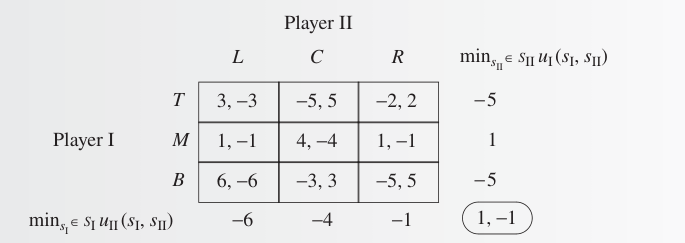
\includegraphics[scale=0.75]{images/2023-10-10-game_theory_50.png}
\end{figure}

In this example, $\underline{v}_I = 1$ and $\underline{v}_{II} =-1$. The maxmin strategy of Player I is M and that of Player II is R. The strategy pair (M, R) is also the equilibrium of this game. In other words, here we have a case where the vector of maxmin strategies is also an equilibrium point: the two concepts lead to the same result.

Since the payoffs $u_I$ and $u_{II}$ satisfy $u_I + u_{II} = 0$, we need to consider only the function $u$, with $u_I = u$ and $u_{II} =-u$. The function $u$ will be termed the payoff function of the game, and it represents the payment that Player II makes to Player I.

Player I, who is usually the row player, seeks to maximize $u(s)$ (his payoff) and Player II, who is usually the column player, is trying to minimize $u(s)$, which is what he is paying (since his payoff is $- u(s)$).

Consider now the maxmin values of the players in a two-player zero-sum game. Player I’s maxmin value is given by

\bee
\underline{v}_I = \max_{s_I \in S_I} \min_{s_{II} \in S_{II}} u(s_I, s_{II})
\eee

and Player II’s maxmin value is

\bee
\underline{v}_{II} = \max_{s_{II} \in S_{II}} \min_{s_{I} \in S_{I}} - u(s_I, s_{II}) = - \min_{s_{II} \in S_{II}} \max_{s_{I} \in S_{I}} u(s_I, s_{II})
\eee

Denote

\begin{align*}
\underline{v} &= \max_{s_I \in S_I} \min_{s_{II} \in S_{II}} u(s_I, s_{II}), \\
\bar{v} &= \min_{s_{II} \in S_{II}} \max_{s_{I} \in S_{I}} u(s_I, s_{II})
\end{align*}

The value $\underline{v}$ is called the maxmin value of the game, and $\bar{v}$ is called the minmax value. Player I can guarantee that he will get at least $\underline{v}$, and Player II can guarantee that he will pay no more than $\bar{v}$. A strategy of Player I that guarantees $\underline{v}$ is termed a maxmin strategy. A strategy of Player II that guarantees $\bar{v}$ is called a minmax strategy.

The maxmin value $\underline{v}$ and the minmax value $\bar{v}$ may be unequal, but it is always the case that $\underline{v} \leq \bar{v}$. The inequality is clear from the definitions of the maxmin and minmax: Player I can guarantee that he will get at least $\underline{v}$, while Player II can guarantee that he will not pay more than $\bar{v}$. As the game is a zero-sum game, the inequality $\underline{v} \leq \bar{v}$ must hold.

\begin{definition}
A two-player game has a value if $\underline{v} = \bar{v}$. The quantity $v = \underline{v} = \bar{v}$ is then called the value of the game. Any maxmin and minmax strategies of Player I and Player II respectively are then called optimal strategies.
\end{definition}

The following two theorems establish a close relationship between the concepts of the value and of Nash equilibrium in two-player zero-sum games.

\begin{theorem}
If a two-player zero-sum game has a value $v$, and if $s^\star_{I}$ and $s^\star_{II}$ are optimal strategies of the two players, then $s^\star = (s^\star_{I}, s^\star_{II})$ is an equilibrium point with payoff $(v, -v)$.

If $s^\star = (s^\star_{I}, s^\star_{II})$ is an equilibrium of a two-player zero-sum game, then the game has a value of $v = u(s^\star_{I}, s^\star_{II})$, and the strategies $s^\star_{I}$ and $s^\star_{II}$ are optimal strategies.
\end{theorem}


%%% Local Variables:
%%% mode: latex
%%% TeX-master: "journal"
%%% End:
